\documentclass[a4paper]{article}
\usepackage[warn]{mathtext}
\usepackage[utf8]{inputenc}
\usepackage[T2A]{fontenc}
\usepackage[english,russian]{babel}
\usepackage{indentfirst}
\usepackage{misccorr}
\usepackage{subcaption}
\captionsetup{compatibility=false}
\usepackage{geometry}
\geometry{verbose,a4paper,tmargin=2cm,bmargin=2cm,lmargin=1.5cm,rmargin=1.5cm}
\usepackage{graphicx}
\usepackage{wrapfig}
\usepackage{amsmath}
\usepackage{fancyhdr}
\usepackage{floatflt}
\usepackage{float}
\usepackage{amssymb}
\usepackage{color}
\usepackage{lscape}
\usepackage{hvfloat}
\usepackage{amsfonts}
\usepackage{euscript}
\usepackage{newunicodechar}
\usepackage{booktabs}


\begin{document}

\pagestyle{fancy} 
\fancyhead[R]{Спектр $H$ и $I$}
\fancyhead[L]{Квантовая физика}
\fancyhead[C]{}
\fancyfoot[C]{ \noindent\rule{\textwidth}{0.4pt} \thepage }

\begin{titlepage}
	\centering
	\vspace{5cm}
    {\scshape\LARGE Московский физико-технический институт\par}
    

	\vspace{3cm}
	{\scshape\Large Лабораторная работа по общей физике \par}
	\vspace{1cm}
    {\huge\bfseries  2.2, 2.3 Изучение спектров атомов водорода и молекулярного спектра йода\par}
	\vspace{1cm}
	\vfill
\begin{flushright}
	{\large выполнила студентка Б01-907}\par
	\vspace{0.3cm}
	{\LARGE Юлия Прохорова}
\end{flushright}

	
	\vfill
Долгопрудный, 2021
% Bottom of the page
\end{titlepage}


\section{Цель работы}
    Исследование спектральных закономерностей в оптическом спектре водорода, спектра поглощения паров йода в видимой области;
    вычисление постоянной Ридберга для водорода по результатам измерения, энергии колебательного кванта молекулы йода и энергию диссоциации в основном и возбужденном состояниях.


\section{В работе используются}
    Стеклянно-призменный монохроматор-спектрометр УМ-2, неоновая лампа, ртутная лампа ПРК-4 для градуировки, водородная лампа, кювета с кристаллами йода.


\section{Теоретические положения}
\subsection{Водород}
Длины волн спектральных линий водородоподобного атома описываются формулой
\begin{equation}
    \frac{1}{\lambda_{mn}} = RZ^2(\frac{1}{n^2} - \frac{1}{m^2}),
\end{equation}
где $R$ - постоянная Ридберга, а $m, n$ -  целые числа. \par
Использование постулатов Бора с учётом кулоновского взаимодействия между ядром и электроном 
позволяет легко определить возможные энергетические состояния водородоподобного атома. Если 
считать ядро неподвижным, то эти энергетические состояния определяются выражением
\begin{equation}
    E_n = -\frac{2 \pi^2 m_e e^4 Z^2}{h^2} \frac{1}{n^2}
\end{equation}


Знание энергетических состояний атома позволяет в соответствии с формулой (2) определить 
возможные частоты его излучения и объяснить наблюдаемые закономерности. \par
В данной работе изучается серия Бальмера, линии которой лежат в видимой области, и изотопический 
сдвиг между линиями водорода. Для серии Бальмера в формуле (1) $n = 2$. Величина $m$ для первых 
четырёх линий этой серии принимает значение 3, 4, 5, 6. \par

\begin{figure}[H]
    \begin{center}
    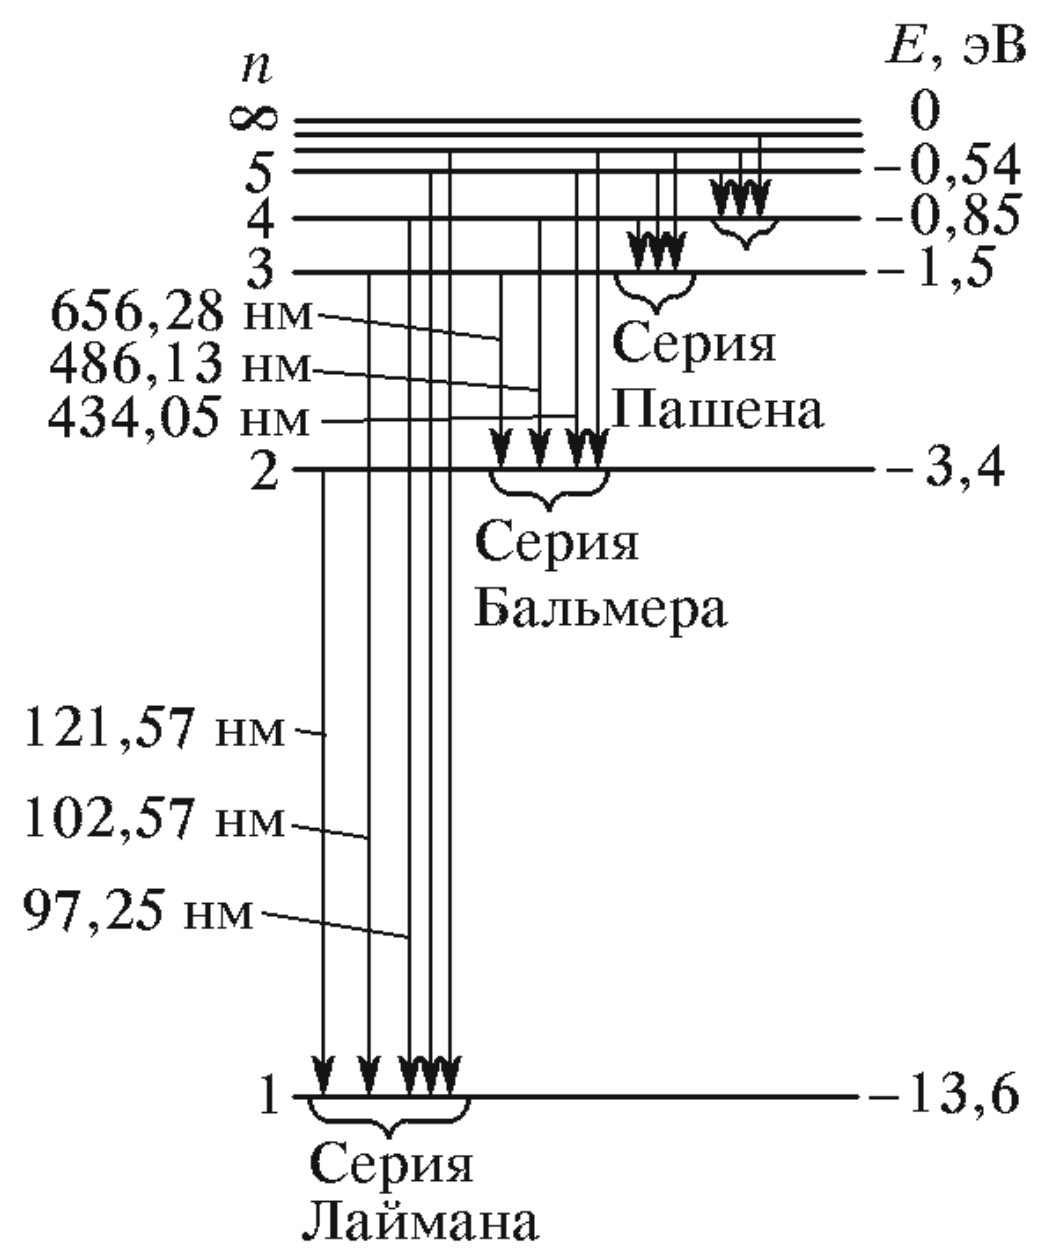
\includegraphics[scale = 0.3]{p1.png}
    \caption{}
    \label{p1}
    \end{center}
\end{figure}

Боровский радиус (радиус первой орбиты) для электрона в поле ядра с зарядом $Z$:
\begin{equation}
    r_B = \frac{\hbar^2}{Z m_e e^2}
\end{equation}
Энергия основного состояния:
\begin{equation}
    E = -\frac{m_e e^4}{2 \hbar^2}Z^2 = -R Z^2
\end{equation}
Аналогичным образом могут быть найдены энергии возбуждённых состояний. Дискретные значения 
энергии электрона в атоме получаются из того условия, что на длине орбиты, по которой движется 
электрон, должно укладываться целое число волн де Бройля. Если радиус орбиты равен $r$, то $n$-му 
состоянию электрона соответствует условие 
\begin{equation}
    2 \pi r = \lambda n (n \in \mathbb{N}) ; m_e v_n = \frac{nh}{2 \pi r}
\end{equation}

Аналогично пп. (3)-(4):
\begin{equation}
     r_B = \frac{n^2 \hbar^2}{Z m_e e^2}
\end{equation}

\begin{equation}
    E = -\frac{m_e e^4}{2 \hbar^2} \frac{1}{n^2} Z^2 = -R \frac{Z^2}{n^2}
\end{equation}

\subsection{Йод}

Молекулы обладают более багатым спектром возбужденных состояний, чем изолированные атомы:
$$E = E_{\text{эл}} + E_{\text{колеб}} + E_{\text{вращ}}$$

Соотношения соответствующих частот:
$$\omega_{\text{эл}} : \omega_{\text{колеб}}: \omega_{\text{вращ}} \approx 1 : \sqrt{
    \frac{m}{M}} : \frac{m}{M} \approx 1 : 10^{-3} : 10^{-6}
$$

Оптические переходы связаны с излучением/поглощением квантов света сопровождаются изменением вращательного
и колебательного состояний. Идет наложение колебательного спектра на электронный:

\begin{figure}[H]
    \begin{center}
    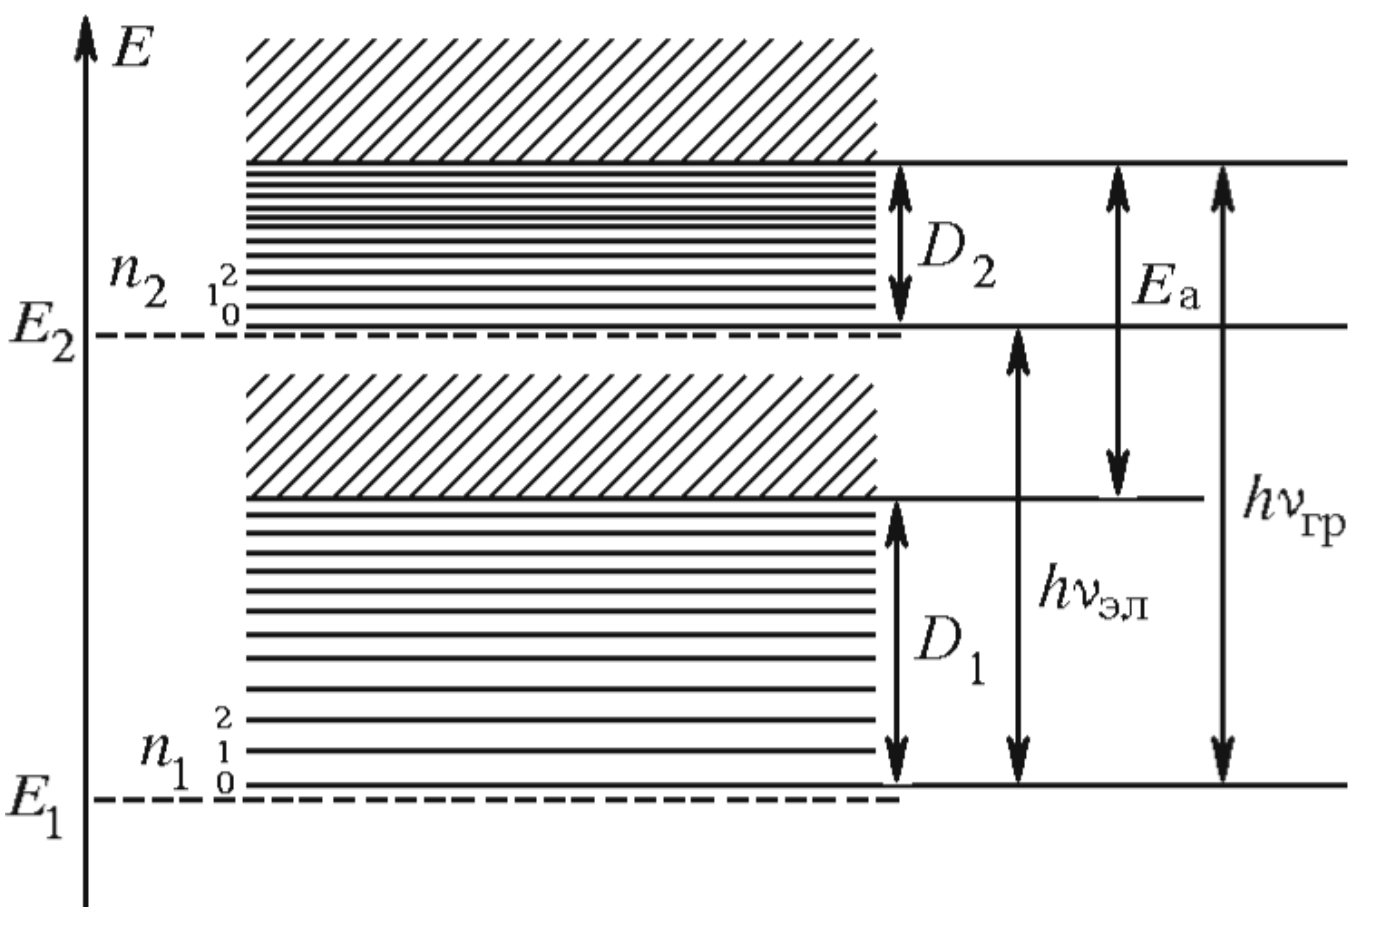
\includegraphics[scale = 0.3]{p4.png}
    \caption{Электронные и электронно-колебательные энергиетические уровни}
    \label{p4}
    \end{center}
\end{figure}

$E_A$ - энергия возбуждения атома возникающая при переходе молекулы из состояния 1 в область 
непрерывного спектра 2. \par
Энергия чисто электронного перехода $h\nu_{\text{эл}} = E_2 - E_1$\par
Граница схождения спектра, где происзодит переход молекулы в облатсь непрерывного спектра $h\nu_{\text{гр}}$\par

Все возможные линии поглощения для переходов между колебательными уровнями, налагающихся
на два соседних электронных состояния можно на серии , соответствующие одному и тому же
начальному состоянию. Эти серии называются сериями Деландра.


\begin{figure}[H]
    \begin{center}
    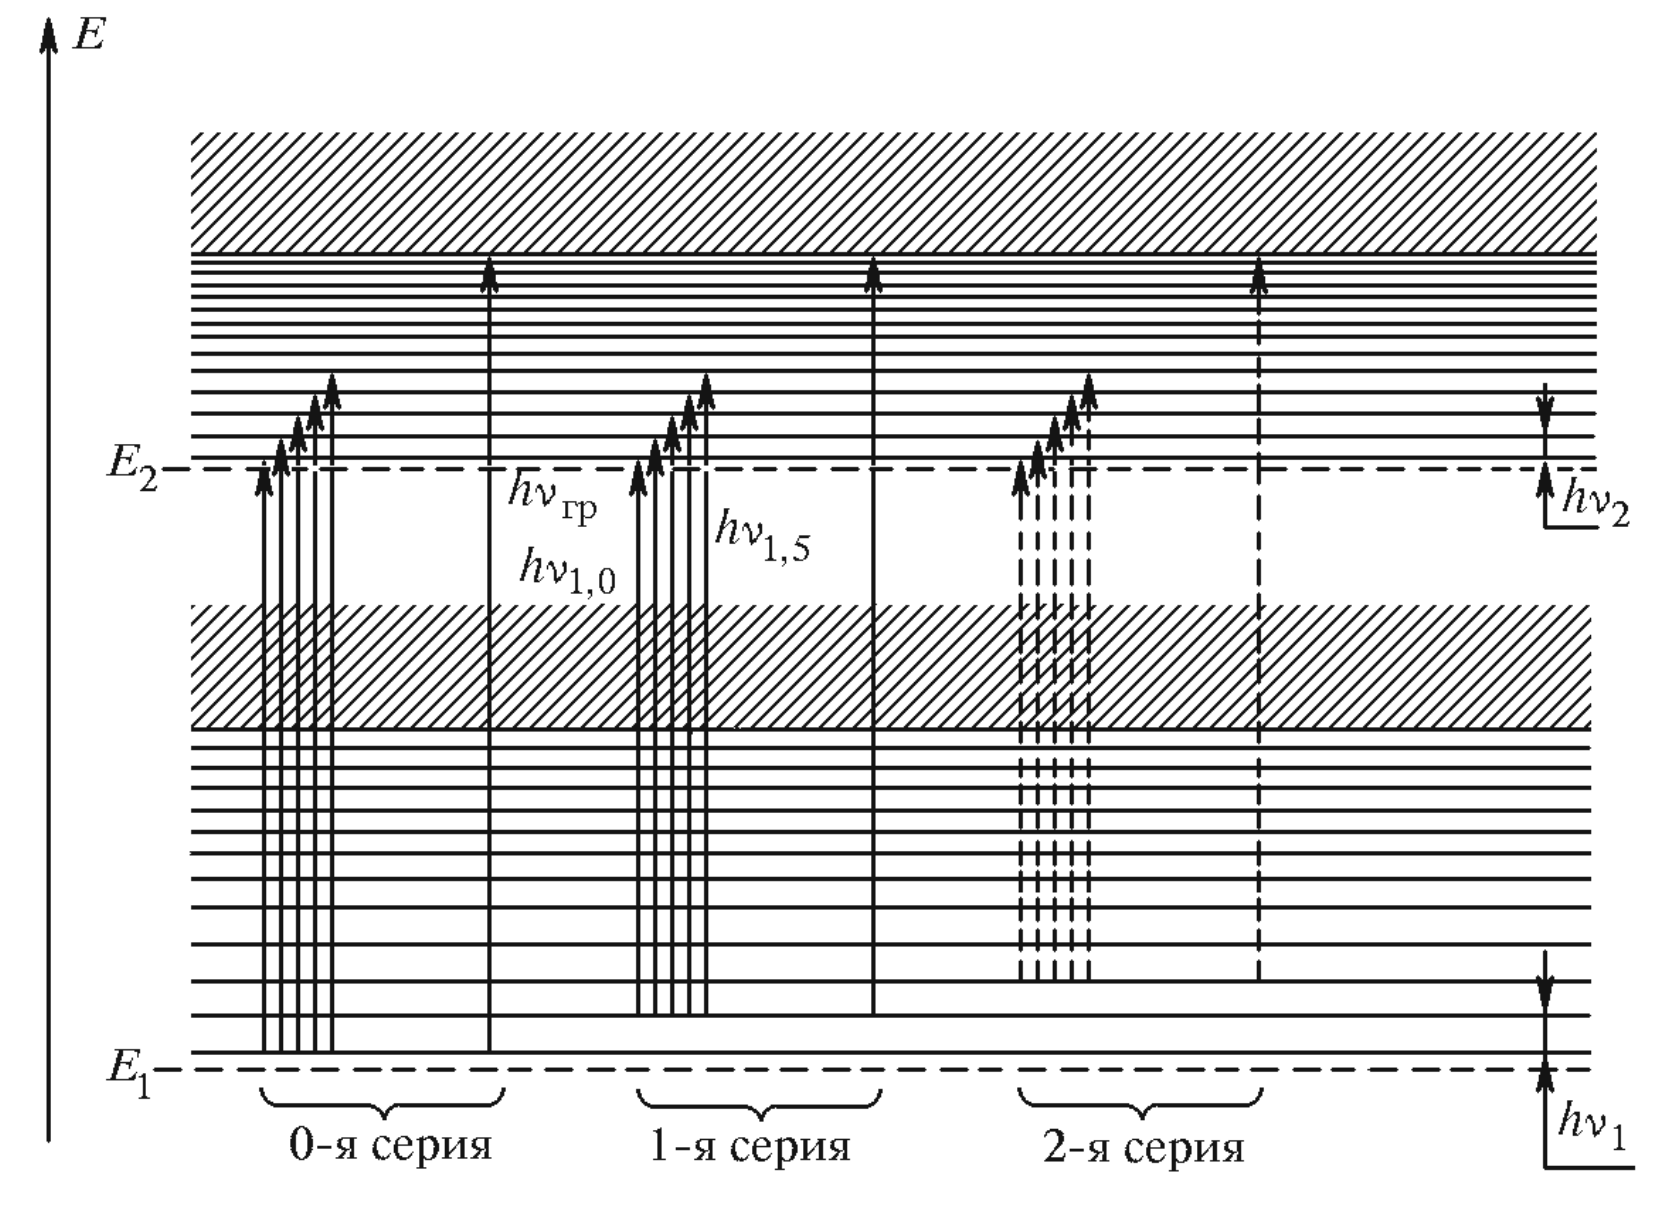
\includegraphics[scale = 0.3]{p5.png}
    \caption{Структура электронно-колебательного спеткра поглощения молекулы йода}
    \label{p5}
    \end{center}
\end{figure}

Для наблюдения таких серий необходимо достаточно много молекул в начальном состоянии.\par

Соотношения интенсивностей серий деландра пропорционально количеству молекул:
$$N_0 : N_1 : N_2 \approx 1 : 1/3 : 1/10$$

Энергетическое положение линий полгощения описывается выражением:
$$h\nu_{0,n_2} = (E_2 - E_1) + h\nu_2 (n_2+1/2) - 1/2 h\nu_1$$
Здесь пренебрегли ангармонизмом, для начальных серий можно пренебреч и энерг. расстояние между сериями:
$$h\nu_{0,n_2} - h\nu_{0,(n_2 - 1)} \approx h\nu_2$$
То есть равны колебательному кванту в возбужденном электронном состоянии.\par

Вся 1-я серия сдвинута в сторону меньших энергий на величину $h\nu_1$ на величину колебательного кванта основног состояния.

\begin{figure}[H]
    \begin{center}
    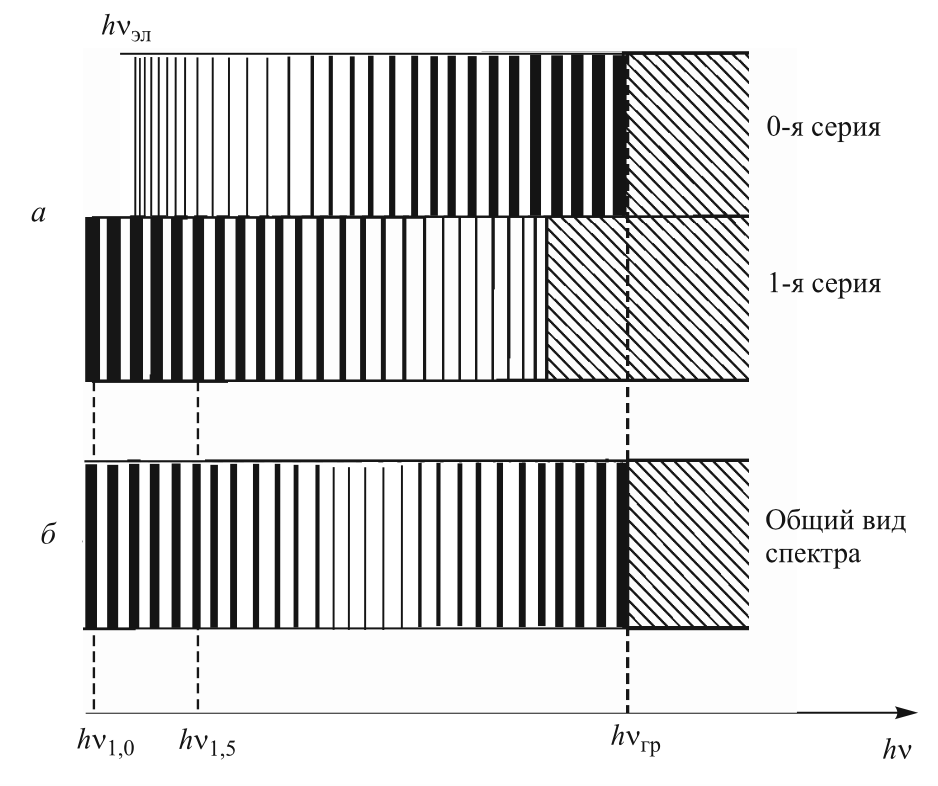
\includegraphics[scale = 0.38]{p6.png}
    \caption{Спектр поглощения паров йода}
    \label{p6}
    \end{center}
\end{figure}


\section{Экспериментальная установка}
Для измерения длин волн спектральных линий в работе используется стеклянно-призменный 
монохроматор-спектрометр УМ-2, предназначенный для спектральных исследований в диапазоне 
от 0,38 до 1 мкм

\begin{figure}[h]
	\begin{center}
	\begin{minipage}[h]{0.45\linewidth}
	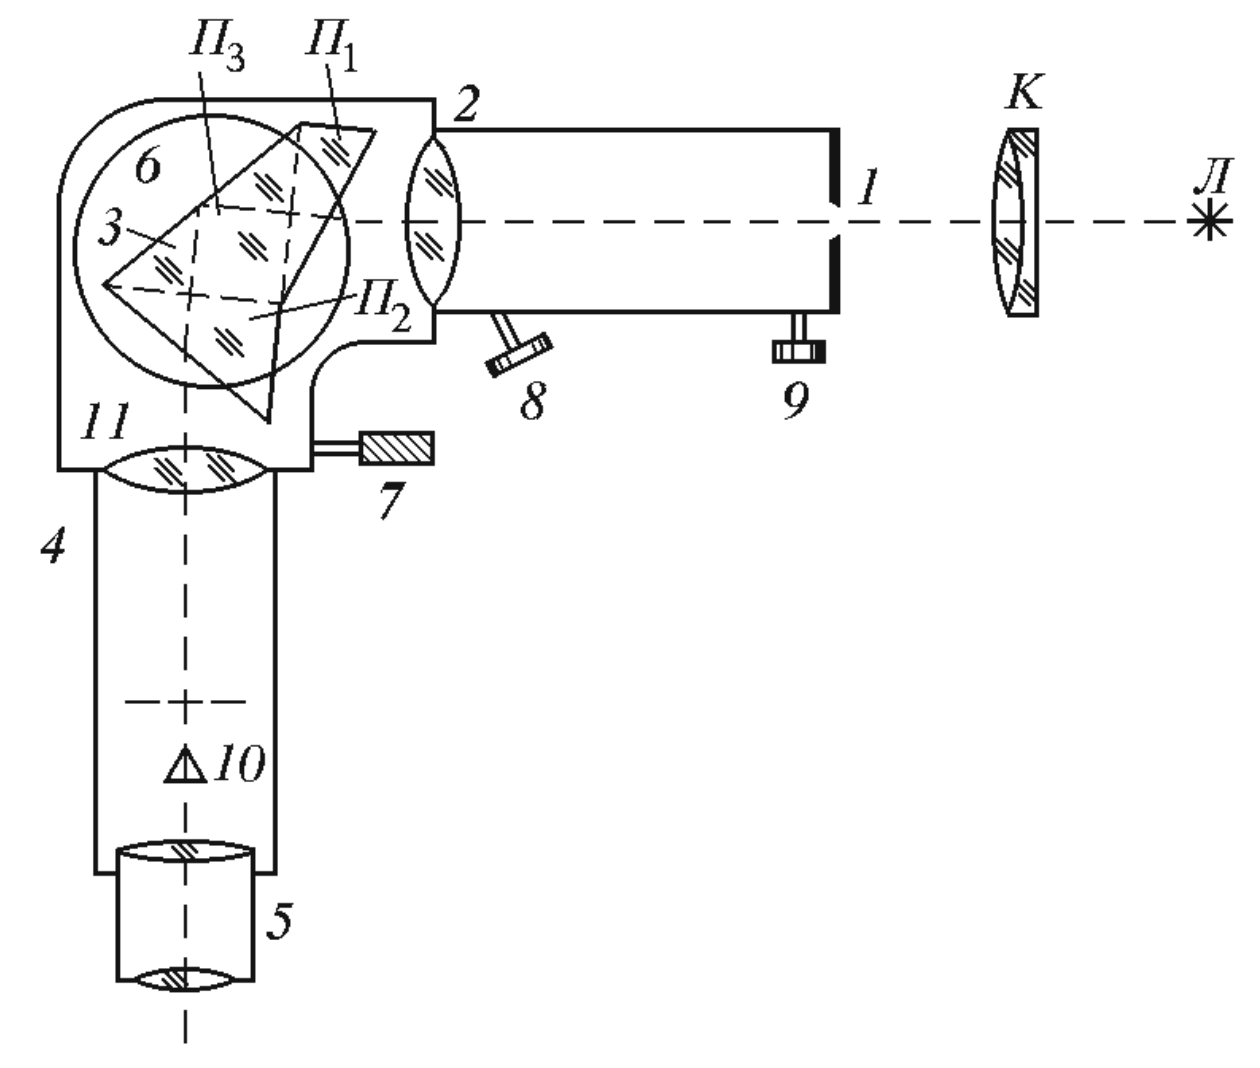
\includegraphics[width=1\linewidth]{p2.png}
	\caption{Установка для Водорода} 
	\label{p2}
	\end{minipage}
	\hfill 
	\begin{minipage}[h]{0.45\linewidth}
	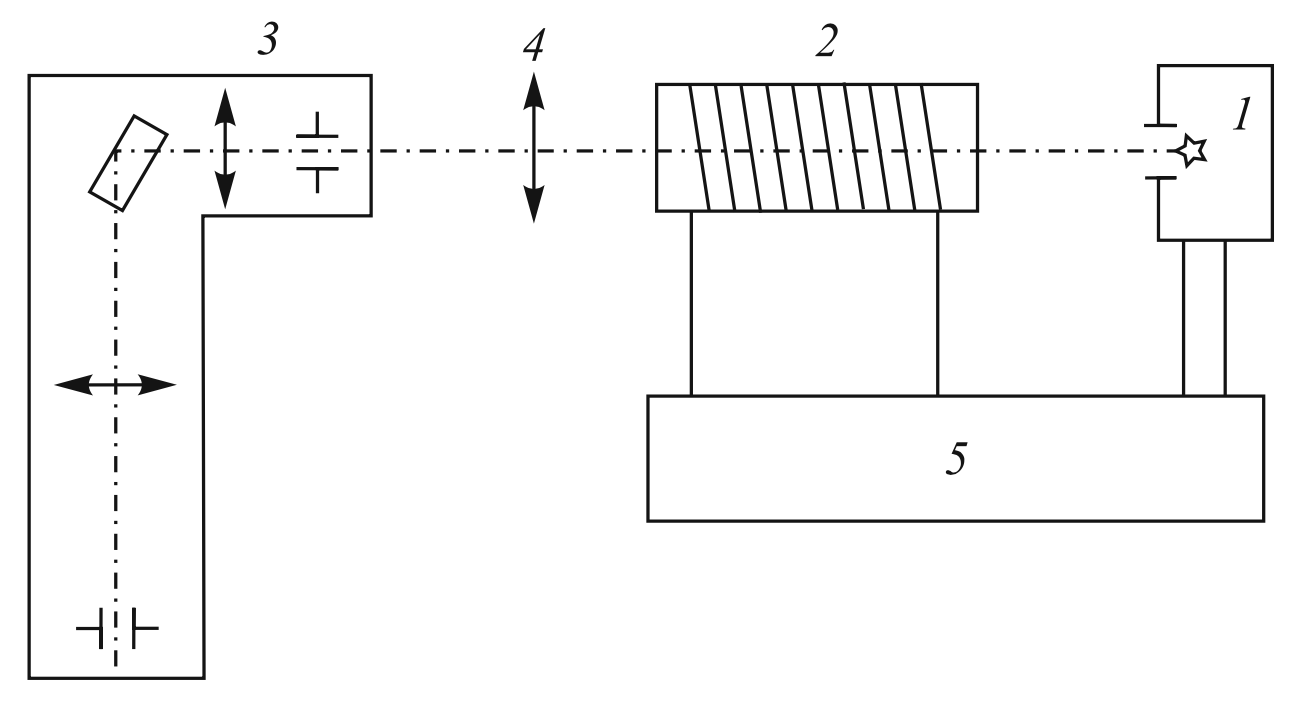
\includegraphics[width=1\linewidth]{p3.png}
	\caption{Установка для Йода}
	\label{p3}
	\end{minipage}
	\end{center}
\end{figure}

Спектрометр нуждается в дополнительной градуировке, проводящейся по спектрам неоновой и ртутной ламп с 
известными длинами волн спектральных линий.

\section{Выполнение работы}
\begin{enumerate}
    \item Выполним градуировку по неоновой и ртутной лампе:
    
    \begin{table}[h]
        \centering
        \begin{tabular}{|l|l|l|l|}
        \hline
        Neon  $\lambda,\; \mathring{A}$ & Neon, $^{о}C$ &  Neon  $\lambda,\; \mathring{A}$     &  Neon, $^{о}C$    \\ \hline
        5331    & 2182    & 6267 & 2690 \\ \hline
        5341    & 2193    & 6305 & 2705 \\ \hline
        5401    & 2232    & 6334 & 2716 \\ \hline
        5852    & 2498    & 6383 & 2736 \\ \hline
        5882    & 2515    & 6402 & 2741 \\ \hline
        5945    & 2548    & 6507 & 2780 \\ \hline
        5976    & 2561    & 6533 & 2792 \\ \hline
        6030    & 2587    & 6599 & 2814 \\ \hline
        6074    & 2606    & 6678 & 2842 \\ \hline
        6096    & 2616    & 6717 & 2856 \\ \hline
        6143    & 2635    & 6929 & 2919 \\ \hline
        6164    & 2644    & 7032 & 2948 \\ \hline
        6217    & 2670    &      &      \\ \hline
        \end{tabular}
        \caption{Градуировка по неоновой лампе}
        \end{table}

        \begin{table}[H]
            \centering
            \begin{tabular}{|l|l|}
            \hline
            Hg, A & Hg   \\ \hline
            4047  & 620  \\ \hline
            4358  & 1169 \\ \hline
            4916  & 1845 \\ \hline
            5461  & 2272 \\ \hline
            5770  & 2452 \\ \hline
            5791  & 2463 \\ \hline
            6234  & 2673 \\ \hline
            6907  & 2910 \\ \hline
            \end{tabular}
            \caption{Градуировка по ртутной лампе}
            \end{table}
    

    \item Построим градуировочную кривую и запишем полученную зависимость:
    $$\lambda = 8,4\cdot10^{-17}\cdot\phi^6-8,8\cdot10^{-13}\cdot\phi^5+3,8\cdot10^{-9}\cdot\phi^4-8,5\cdot10^{-6}\cdot\phi^3+10^{-2}\cdot\phi^2-5,7\cdot\phi+5,2\cdot10^3$$

    \begin{figure}[H]
        \begin{center}
        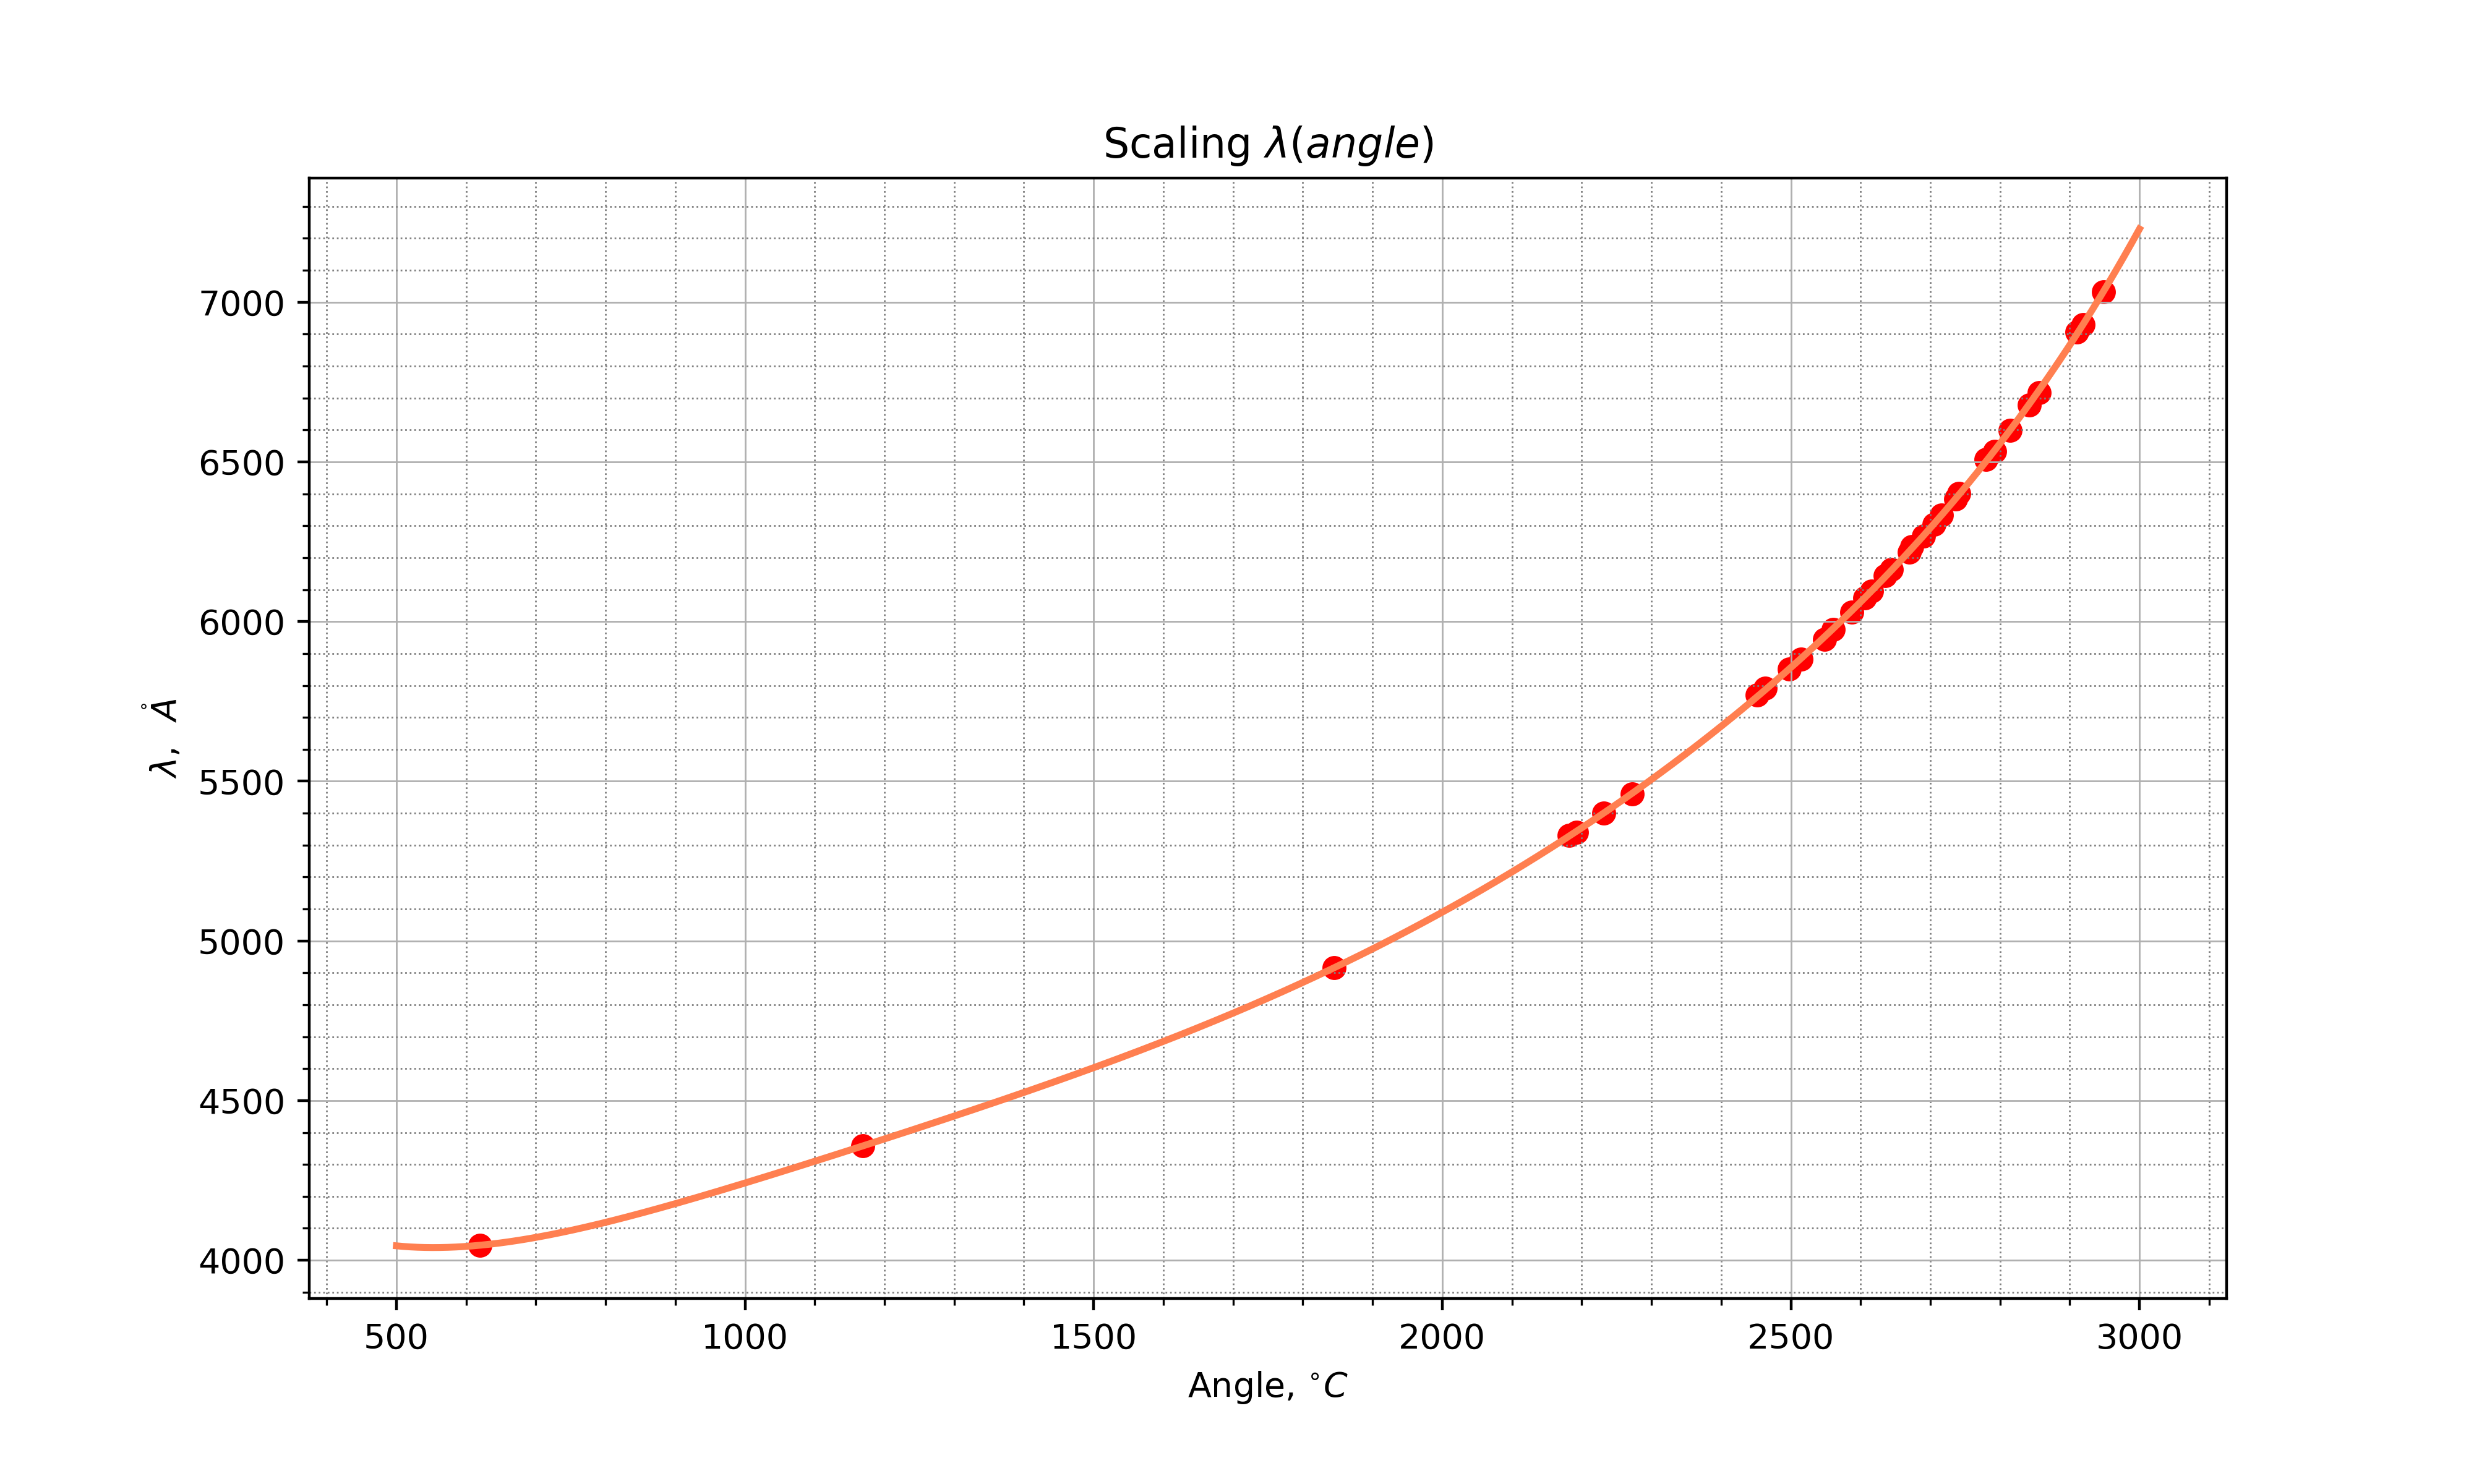
\includegraphics[scale = 0.6]{Scale.png}
        \caption{Градуировка по неону и ртути }
        \label{Neon}
        \end{center}
    \end{figure}


    \item По градуировочным графикам определим длины волн $H_{\alpha}, H_{\beta}, H_{\gamma}, H_{\delta}$

    \begin{table}[htb]
        \centering
        \begin{tabular}{|c|c|c|}
            \hline
            H line & H angle $^{\circ}$ &  $\lambda, \; \mathring{A}$  \\
            \hline 
            $H_{\alpha}$ & 2800 & 6558,1  \\\hline
            $H_{\beta}$ & 1790 & 4860,0  \\\hline
            $H_{\gamma}$& 1142 & 4339,1\\\hline
            $H_{\delta}$ & 716 & 4078,0 \\ \hline

        \end{tabular}
    \end{table}

    
    \item По формуле $\frac{1}{\lambda_{mn}} = RZ^2(\frac{1}{n^2} - \frac{1}{m^2})$ определим постоянные Ридберга:
    $$R_\alpha = 109787,9 см^{-1} $$
    $$R_\alpha = 109739,4 см^{-1} $$
    $$R_\alpha = 109744,1 см^{-1} $$
    $$R_\alpha = 110348,2 см^{-1} $$

    Усредним $R = 109904,9 \pm 256,6 см^{-1}$

    \item По градуировочной кривой определим длины волн поглащения йода\par
    $n_{1,0} - 2656^{\circ} - 6187,6 \; \mathring{A}$ - самая длиноволновая\par
    $n_{1,5} - 2551^{\circ} - 5958,0\; \mathring{A}$ - 6-я по счету слева\par
    $n_{\text{гр}} - 1973^{\circ} - 5057,9 \; \mathring{A}$ - граница схождения спектра\par
    \item Вычислим в электронвольтах энергию колебательного кванта возбужденного состояния молекулы йода:\par
    $h\nu_2 = (h\nu_{1,5} - h\nu_{1,0})/5 = 0.0155$ (эВ)
    \item Используя $h\nu_1 = 0.027$(эВ) и энергию возбуждения атома $E_A = 0.94$(эВ) $h\nu_{\text{гр}} \approx 2.45$(эВ)  $h\nu_{1,0} \approx 1.93$(эВ) вычислим:
    \begin{itemize}
        \item Энергию электронного перехода $h\nu_{\text{эл}} = h\nu_{1,0} + h\nu_1 \approx 2,03$ (эВ)
        \item Энергия диссоциации из основного состояния $D_1 = h\nu_{\text{гр}} - E_A \approx 1.52$ (эВ)
        \item Энергия диссоциации из возбужденного состояния $D_2 = h\nu_{\text{гр}} - h\nu_{\text{эл}} \approx 0.42$ (эВ)
    \end{itemize}
     
\end{enumerate}

\section{Вывод}
В данной работе исследованы сериальные закономерности в оптических спектрах водорода и йода. 
Вычислена постоянная Ридберга для водорода по результатам измерения. Вычислена энергия колебательного 
кванта молекулы йода и энергия диссоциации в основном и возбужденном состояниях.

\end{document}